\documentclass{article}

\date{24 Novembre 2024}
\usepackage[nb-sem=9, auteurs={Kylian Boyet, George Ober, Hugo Vangilluwen, Felix Rondeau}]{../kholles}

\begin{document}

\maketitle

\begin{question_kholle}[]{Montrer que si $A$ et $B$ sont deux parties non vides majorées de $\R$, alors $\sup(A+B) = \sup A + \sup B$}
  Soient $A$ et $B$ deux parties non vides et majorées de $\mathbb{R}$. On note $A+B$ l'ensemble
  $$
    A+B = \{ a+b \mid (a, b) \in A\times B \}
  $$
  C'est aussi une partie non vide de $\mathbb{R}$.\\
  Soit $x \in (A+B)$ fixé quelconque. Par définition de $A+B$, $\exists(a, b) \in A\times B : x=a+b$

  $$
    \left. \begin{array}{ll}
      a \leqslant \sup A \\
      b \leqslant \sup B
    \end{array}\right\} \implies x = a+b \leqslant \sup A + \sup B
  $$
  donc $\sup A+\sup B$ est un majorant de $A+B$. Ainsi, comme l’ensemble $A+B$ est une partie non vide et majorée de \R, il admet une borne supérieure, plus petite que tous les majorants et en particulier que $\sup A+\sup B$:
  $$\sup(A+B) \leqslant \sup A + \sup B$$
  De plus, $\sup(A+B)$ est un majorant de $A+B$ donc, pour $(a, b) \in A\times B$ fixés, on a
  $$
    a+b \leqslant \sup (A+B) \iff a \leqslant \sup(A+B) -b
  $$
  en relâchant le caractère fixé de $a$, on a
  $$
    \forall a \in A, a\leqslant \sup(A+B) - b
  $$
  donc $\sup(A+B) - b$ est un majorant de $A$, donc plus petit que $\sup A$, d'où

  $$
    \sup A \leqslant \sup(A+B) - b \iff b \leqslant \sup(A+B) - \sup A
  $$
  Donc en relâchant le caractère fixé de $b$ on a
  $$
    \forall b \in B, b\leqslant \sup(A+B) - \sup A
  $$
  donc $\sup(A+B) - \sup A$ est un majorant de $B$ donc plus petit que $\sup B$
  d'où

  $$
    \sup B \leqslant \sup(A+B) - \sup A \iff \sup A + \sup B \leqslant \sup (A+B)
  $$
  Ainsi, par double inégalité
  $$
    \sup A + \sup B = \sup (A+B)
  $$

\end{question_kholle}

\begin{question_kholle}{Preuve de la caractérisation de la propriété de la borne supérieure dans \R avec des $\varepsilon$}
  \hfill\\
  \begin{description}
    \item[$(\implies)$] Supposons que $\sigma =\sup A$.
          \begin{itemize}
            \item Par définition, la borne supérieure est le plus petit majorant donc $\forall a\in A, \leq \sigma$.
            \item Soit $\varepsilon\in\R_{+}^{*}$ fixé quelconque. Par l’absurde, supposons que pour tout $a\in A$, $\sigma-\varepsilon\geq a$.\\
                  Alors, $\sigma-\varepsilon\geq \sup A=\sigma$ d’où $-\varepsilon\geq 0$ ce qui contredit la définition de $\varepsilon$.
          \end{itemize}
          Ainsi, $\exists a\in A: \sigma-\varepsilon<a$.

    \item[$(\impliedby)$] Supposons
          \begin{numcases}{}
            \forall a\in A, a\leq \sigma \label{10:2:hyp1}\\
            \forall \varepsilon\in\R_{+}^{*}, \exists a\in A: \sigma-\varepsilon<a \label{10:2:hyp2}
          \end{numcases}
          \begin{itemize}
            \item $\sigma\in M(A)$ par conséquence directe de \eqref{10:2:hyp1}
            \item $\sigma$ est plus petit que tout autre majorant:\\
                  Soit $M\in M(A)$ fixé quelconque. Par l’absurde, supposons que $M<\sigma$. Appliquons \eqref{10:2:hyp2} pour $\varepsilon\leftarrow \sigma - M$ (ce qui est autorisé car $M<\sigma$ donc $\sigma-M>0$):
                  \[
                    \exists a_{0}\in A: \sigma-(\sigma-M)<a_{0}
                  \]
                  Donc $M<a_{0}$ ce qui contredit $M\in M(A)$. Ainsi, $\sigma\leq M$, si bien que $M(A)$ admet $\sigma$ comme plus petit élément donc $A$ admet $\sigma$ comme borne supérieure.
          \end{itemize}
  \end{description}
\end{question_kholle}

\begin{question_kholle}
  [\noindent Soient $(A, B) \in \mathcal{P}(\R)^2$ fq. \\
    \textit{Définition de la densité}
    \begin{align}
      A \text{ est dense dans } B
      \text{ si } \left\{ \begin{array}{ll}
                            A \subset B \\
                            \mathrm{et} \\
                            \forall (u,v) \in \R^2, B \cap {]}u;v{[} \neq \emptyset \implies A \cap  {]}u;v{[} \neq \emptyset
                          \end{array} \right.
    \end{align}
    \textit{Caractérisation de la densité par les $\varepsilon$}
    \begin{align}
      A \text{ est dense dans } B
      \iff \left\{ \begin{array}{ll}
                     A \subset B \\
                     \mathrm{et} \\
                     \forall b \in B, \forall \varepsilon \in \R_+^*, \exists a \in A: |b-a|< \varepsilon
                   \end{array} \right.
    \end{align}
  ]
  {Preuve de la caractérisation de la densité}

  \textit{Montrons la caractérisation de la densité}\\
  \emph{Sens Direct} Supposons $A$ dense dans $B$
  \begin{itemize}[label=\textemdash]
    \item Par déf $A \subset B$
    \item Soit $b \in B$ et $\varepsilon \in \R_+^*$ fq

          Appliquons le (ii) de la déf de Densité pour $u \leftarrow b - \varepsilon$ et $v \leftarrow b + \varepsilon$
          $$B \cap ]b - \varepsilon, b + \varepsilon[ \neq \emptyset \implies A \cap ]b - \varepsilon,  b + \varepsilon[ \neq \emptyset$$
            Or, $B \cap ]b - \varepsilon, b + \varepsilon[ \neq \emptyset$ est vraie
              donc $A \cap ]b - \varepsilon,  b + \varepsilon[ \neq \emptyset$

              Ce qui permet de choisir $a \in A \cap ]b - \varepsilon,  b + \varepsilon[$.
              Un tel $a$ vérifie $a \in A$ et $a \in ]b - \varepsilon,  b + \varepsilon[ \iff |b-a| < \varepsilon$
  \end{itemize}
  \bigbreak
  \noindent \emph{Sens réciproque.} Supposons
  \[
    \left\{\begin{array}{ll} A \subset B \\\mathrm{et}\\ \forall b \in B, \forall \varepsilon \in \R_+^*, \exists a \in A: |b-a|< \varepsilon \end{array}\right.
  \]

  \begin{itemize}
    \item On a donc $A \subset B$
    \item Soient $(u, v) \in \R^2$ fq tq $B \cap ]u, v[ \neq \emptyset$

                  Soit $b \in B \cap ]u, v[$ fq.
                  Appliquons l'hypothèse pour $b\leftarrow b$ et $\varepsilon \leftarrow \min\{v - b, b - u\}$, qui est autorisé $v-b$ et $b-u$ sont positifs

                  Donc $\exists a \in A: | b - a| < \varepsilon $

                  Fixons un tel a, alors:
                  $$
                    b-\varepsilon < a < b + \varepsilon
                  $$

                  Donc $$
                    \left\{\begin{array}{ll}
                      a < b + \varepsilon = b + \underbrace{\min\{v - b, b - u\}}_{\leqslant v - b} \leqslant b + v - b = v \\ \mathrm{et}\\
                      a > b - \varepsilon = b - \underbrace{\min\{v - b, b - u\}}_{\leqslant b - u} \geqslant b - (b - u) = u
                    \end{array}\right.
                  $$

                  Donc $a \in ]u, v[$.
  \end{itemize}
  Donc $A \cap ]u, v[ \neq \emptyset$

\end{question_kholle}


\begin{question_kholle}
  {Montrer que \Q et $\R\setminus\Q$ sont denses dans \R}

  Soit $x \in \R$ fq.
  Posons $\forall n \in \N, a_n = \frac{\lfloor2^n x\rfloor}{2^n}$. \\
  Soit $n \in \N$ fq. \\
  \begin{itemize}
    \item $a_n \in \Q$ car $\lfloor2^n x\rfloor \in \Z$ et $2^n \in \N$.
    \item \begin{equation*}
            a_n = \frac{\lfloor2^n x\rfloor}{2^n}
            \implies \frac{2^n x - 1}{2^n} \leqslant a_n \leqslant \frac{2^n x}{2^n}
            \implies x - \frac{1}{2^n} \leqslant a_n \leqslant x
          \end{equation*}
          Or $\nicefrac{1}{2^n} \arrowlim{n}{+\infty} 0$ donc d'après le théorème d'existence de limite par encadrement, \\ $a_n \arrowlim{n}{+\infty} x$.
  \end{itemize}
  Donc d'après la caractérisation séquentielle de la densité, \Q est dense dans \R.
  \bigbreak

  \noindent Soit $x \in \R$ fq. \\
  Alors $x + \sqrt{2} \in \R$.
  D'après la démonstration précédente, $\exists b \in \Q^\N : b_n \arrowlim{n}{+\infty} x + \sqrt{2}$. \\
  Fixons un telle suite $b$.
  Considérons $c = b - \sqrt{2}$. \\
  Soit $n \in \N$ fq.
  \begin{itemize}
    \item $c_n \in \R\setminus\Q$ car $b_n \in \Q$ et $\sqrt{2} \in \R \setminus \Q$.
    \item \begin{equation*}
            \left. \begin{matrix}
              b_n \arrowlim{n}{+\infty} x + \sqrt{2} \\
              c_n = b_n - \sqrt{2}
            \end{matrix} \right\}
            \implies c_n \arrowlim{n}{+\infty} x
          \end{equation*}
  \end{itemize}
  Donc d'après la caractérisation séquentielle de la densité, $\R\setminus \Q$ est dense dans \R.
\end{question_kholle}

\begin{question_kholle}{Caractérisation séquentielle de la densité}
  \hfill\\
  \begin{description}
    \item[$(\implies)$] Supposons que $A$ est dense dans $B$.
          \begin{itemize}
            \item $A\subset B$ par définition.
            \item Soit $b\in B$ fixé quelconque. D’après la caractérisation de la densité appliqué pour $b\leftarrow b$ et $\varepsilon\leftarrow \frac{1}{2^{n}}$
                  \[
                    \exists a\in A: |b-a|\leq \frac{1}{2^{n}}
                  \]
                  Notons un tel $a$ $a_{n}$. On vient de construire la suite $(a_{n})\in A^{\N}$ telle que
                  \[
                    \forall n\in N, |b-a_{n}|\leq \frac{1}{2^{n}}\\
                  \]
                  or $\displaystyle\lim_{n\to +\infty}\frac{1}{2^{n}}=0$ donc, par le théorème sans nom, la suite $(a_{n})_{n\in\N}$ converge vers $b$.
          \end{itemize}
    \item[$(\impliedby)$] Supposons que tout élément de $B$ est limite d’une suite d’éléments de $A$.
          \begin{itemize}
            \item $A\subset B$ par hypothèse.
            \item Soient $\varepsilon\in\R_{+}^{*}$ et $b\in B$ fixés quelconques.
                  Soit $(a_{n})\in A^{\N}$ une suite qui converge vers $b$ (elle existe par hypothèse). Appliquons la définition de sa convergence pour $\varepsilon\leftarrow \frac{\varepsilon}{2}>0$ :
                  \[
                    \exists N\in\N: \forall n\in\N, n\geq N \implies |a_{n}-b|\leq \frac{\varepsilon}{2}
                  \]
                  Fixons un tel $N$. On a alors
                  \[
                    |a_{N}-b|\leq \frac{\varepsilon}{2} \quad \text{donc} \quad |a_{N}-b|<\varepsilon \quad \text{donc} \quad \exists a\in A: |b-a|<\varepsilon
                  \]
          \end{itemize}
  \end{description}
\end{question_kholle}

\begin{question_kholle}[{Soit $A \in \mathcal{P}(\R)$ non vide et majorée. Soit $\sigma \in \R$
        $$
          \sigma = \sup A \iff \left\{ \begin{array}{ll}
            \sigma \in M(A) \\
            \exists (a_{n})_{n \in \N} \in A^{\N} : \lim_{n \to +\infty} a_n = \sigma
          \end{array}\right.
        $$
      }]{Caractérisation séquentielle de la borne supérieure}
  \hfill\\
  \begin{itemize}[label=$\star$]
    \item Supposons que $\sigma = \sup A$.
          \begin{itemize}[label=$\bullet$]
            \item Par définition d'une borne sup, $\sigma \in M(A)$.
            \item Soit $n \in \N$. Appliquons la caractérisation de la borne sup par les epsilon pour $\varepsilon \leftarrow \frac{1}{2^{n}}$.
                  $\exists c \in A : \sigma - \frac{1}{2^{n}} < c \leqslant \sigma$.
                  Fixons un tel $c$ et notons le $a_{n}$. En relâchant le caractère fixé de $n$, on a crée la suite $(a_{n})_{n \in \N}$ telle que
                  $$
                    \forall n \in \N, \sigma - \frac{1}{2^{n}} < a_{n}\leqslant \sigma
                  $$
                  Cette suite converge vers $\sigma$ par encadrement.
          \end{itemize}
    \item Réciproquement, supposons que $\sigma \in M(A)$ et qu'il existe une suite $(a_{n})_{n \in \N}$ d'éléments de $A$ qui converge vers $\sigma$. Montrons que $\sigma = \sup A$ d'après la caractérisation par les $\varepsilon$.
          \begin{itemize}[label=$\bullet$]
            \item$\sigma \in M(A)$
            \item Soit $\varepsilon>0$. Appliquons la définition de la convergence de $a$ pour $\varepsilon \leftarrow \frac{\varepsilon}{2}$

                  $$
                    \exists N \in \N : \forall n \geqslant N, \lvert a_{n} - \sigma \rvert  \leqslant \frac{\varepsilon}{2} \implies \sigma - \frac{\varepsilon}{2}\leqslant a_{n}
                  $$
                  En particulier $a_{N} \in A$ vérifie
                  $$
                    \sigma - \varepsilon < \sigma - \frac{\varepsilon}{2} \leqslant a_{N} \underbrace{ \leqslant }_{ \sigma \in M(A) } \sigma
                  $$
                  Ce qui permet de conclure.
                  Donc $\sigma = \sup A$.
          \end{itemize}
  \end{itemize}
\end{question_kholle}


\begin{question_kholle}[
    Soit u $\in \K ^ \N, (\ell_1, \ell_2) \in \K ^2$
    Si u converge vers $\ell_1$ et $\ell_2$, alors $\ell_1 = \ell_2$
  ]{Preuve de l'unicité de la limite d'une suite convergente}
  Par l'absurde, supponsons que $u$ converge vers $\ell_1$ et $\ell_2$, et $\ell_1 \neq \ell_2$.
  On prendra $\varepsilon_0 = \varepsilon_1 = \varepsilon_2$ assez petit pour que les tubes soient disjoints.\\
  Posons donc $\displaystyle\varepsilon_0 = \frac{|\ell_1 - \ell_2|}{3}$
  \begin{itemize}
    \item Appliquons la définition de la convergence de u vers $\ell_1$, pour $\varepsilon \leftarrow \varepsilon_0$, ce qui est autorisé car $\varepsilon_0 \in \R_+^*$
          \begin{equation}\label{eq:1}
            \exists N_1 \in \N : \forall n \in \N, n \geqslant N_1 \implies |u_n - \ell_1| \leqslant \varepsilon_0
          \end{equation}
          \begin{equation}\label{eq:2}
            \exists N_2 \in \N : \forall n \in \N, n \geqslant N_2 \implies |u_n - \ell_2| \leqslant \varepsilon_0
          \end{equation}
          Fixons de tels $N_1$ et $N_2$.
    \item Posons $n_0 = N_1 + N_2$
          \begin{itemize}
            \item $n_0 \geqslant N_1$, donc (\ref{eq:1}) s'applique: $|u_{n_0} - \ell_1| \leqslant \varepsilon_0$
            \item $n_0 \geqslant N_2$, donc (\ref{eq:2}) s'applique: $|u_{n_0} - \ell_2| \leqslant \varepsilon_0$
          \end{itemize}
    \item \begin{align*}
            |\ell_1 - \ell_2| & = |\ell_1 - u_{n_0} + u_{n_0} - \ell_2|                                                                                         \\
                              & \leqslant \underbrace{|\ell_1 - u_{n_0}|}_{\leqslant \varepsilon_0} + \underbrace{|u_{n_0} - \ell_2|}_{\leqslant \varepsilon_0} \\
                              & \leqslant 2 \frac{|\ell_1 - \ell_2|}{3}                                                                                         \\
            \implies 1        & \leqslant \frac 2 3
          \end{align*}
          Contradiction
  \end{itemize}
  \begin{figure}[H]
    \centering
    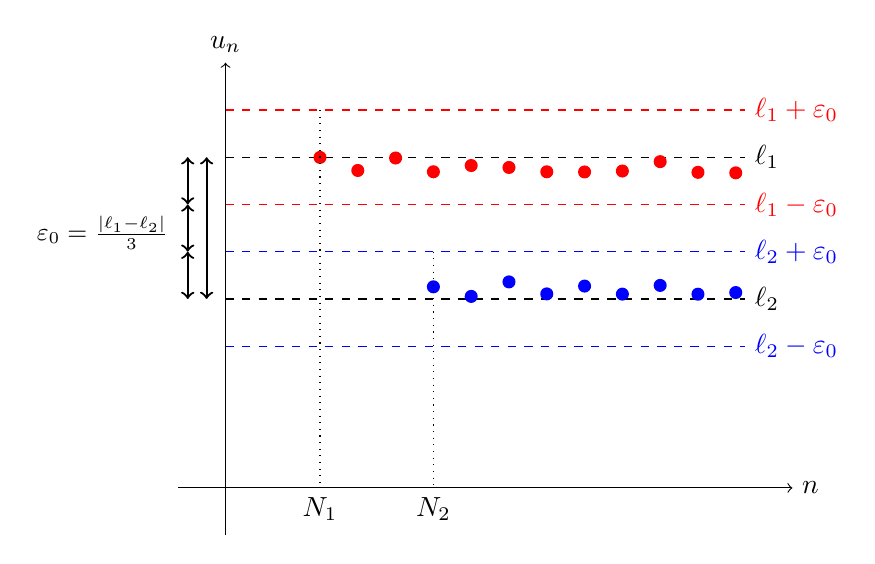
\begin{tikzpicture}[scale=1.2]

      \draw[->] (-0.5, 0) -- (6, 0) node[right] {$n$};
      \draw[->] (0, -0.5) -- (0, 4.5) node[above] {$u_n$};

      \draw[dashed] (0, 3.5) -- (5.5, 3.5) node[right] {$\ell_1$};
      \draw[dashed] (0, 2) -- (5.5, 2) node[right] {$\ell_2$};

      \draw[red,  dashed] (0, 4) -- (5.5, 4) node[right] {$\ell_1 + \varepsilon_0$};
      \draw[red,  dashed] (0, 3) -- (5.5, 3) node[right] {$\ell_1 - \varepsilon_0$};

      \draw[blue,  dashed] (0, 2.5) -- (5.5, 2.5) node[right] {$\ell_2 + \varepsilon_0$};
      \draw[blue,  dashed] (0, 1.5) -- (5.5, 1.5) node[right] {$\ell_2 - \varepsilon_0$};


      \foreach \x in {1, 1.4, 1.8, 2.2, 2.6, 3, 3.4, 3.8, 4.2, 4.6, 5, 5.4} {
          \node[circle, fill=red, scale=0.5] at (\x, {3.4 + 0.1*rand}) {};
        }
      \foreach \x in {2.2, 2.6, 3, 3.4, 3.8, 4.2, 4.6, 5, 5.4} {
          \node[circle, fill=blue, scale=0.5] at (\x, {2.1 + 0.1*rand}) {};
        }


      \draw[<->, thick] (-0.4, 3.5) -- (-0.4, 3);
      \draw[<->, thick] (-0.4, 3) -- (-0.4, 2.5);
      \draw[<->, thick] (-0.4, 2.5) -- (-0.4, 2);
      \draw[<->, thick] (-0.2, 2) -- (-0.2, 3.5);
      \node[left] at (-0.5, 2.7) {\small $\varepsilon_0 = \frac{|\ell_1 - \ell_2|}{3}$};

      \draw[dotted] (1, 4) -- (1, 0) node[below] {$N_1$};
      \draw[dotted] (2.2, 2.5) -- (2.2, 0) node[below] {$N_2$};

    \end{tikzpicture}
    \caption{À partir du rang $n_0$, supérieur à $N_1$ et $N_2$, tous les termes de la suite doivent être contenus dans les deux tubes disjoints, ce qui est impossible.}
  \end{figure}
\end{question_kholle}

\begin{question_kholle}{Toute suite convergente est bornée}

  Soit $u \in \mathbb{K}^{\mathbb{N}}$ convergente.
  Posons $\ell = \lim u$
  Appliquons la définition de la convergence pour $\varepsilon \leftarrow 1$
  $$
    \exists N_{1}\in \mathbb{N}: \forall n \in \mathbb{N}, n \geqslant N_{1} \implies |u_{n}-\ell| \leqslant 1
  $$
  Fixons un tel $N_{1}$
  Posons alors $M = \max\left\{ |u_{0}|, |u_{1}|, |u_{2}| \dots |u_{N_{1}}|, |\ell|+1 \right\}$, qui est bien défini, car toute partie finie, non vide d'un ensemble totalement ordonné (ici $(\mathbb{R}, \leqslant)$) admet un pgE.

  Soit $n \in \mathbb{N}$ fq.
  \begin{itemize}
    \item Si $n \in [\! [0, N_{1}]\!], |u_{n}| \in \left\{ |u_{0}|, |u_{1}|, |u_{2}| \dots |u_{N_{1}}|, |\ell|+1 \right\}$ donc $|u_{n}| \leqslant M$
    \item Sinon,
  \end{itemize}

  \begin{align*}
    n> N_{1} & \implies |u_{n} - \ell| \leqslant 1              \\
             & \implies |u_{n}| - |\ell| \leqslant 1            \\
             & \implies |u_{n}| \leqslant 1+ |\ell| \leqslant M
  \end{align*}

  Ainsi, $\forall n \in \mathbb{N}, |u_{n}| \leqslant M$.
\end{question_kholle}


\pagebreak

\begin{question_kholle}[]{Dans un ensemble totalement ordonné, toute partie finie non vide possède un plus grand élément et un plus petit élément.}
  Soit $(E, \preccurlyeq)$ un ensemble totalement ordonné, considérons pour tour $n \in \mathbb{N}^{*}$ la propriété.
  $$
    \mathcal{H}_{n} : \text{toute partie de }E \text{ de cardinal }n \text{ admet un plus petit et un plus grand élément}
  $$
  \begin{itemize}[label=$\star$]
    \item Initialisation $n \leftarrow 1$

          Soit $A \in \mathcal{P}(E)$ fixée telle que $\lvert A \rvert = 1$
          $A$ est non vide, donc $\exists a \in A : A = \{ a \}$

          $a$ est le plus petit et le plus grand élément, donc $\mathcal{H}_{1}$ est vraie.

    \item Hérédité
          Soit $n \in \mathbb{N}^{*}$ fixé quelconque tel que $\mathcal{H}_{n}$ est vraie.
          Soit $A \in \mathcal{P}(E)$ fixée quelconque tel que $\lvert A \rvert = n+1$
          $$
            A \neq \emptyset \implies \exists a \in A : A = (A \setminus \{ a \}) \cup \{ a \}
          $$
          Or, $\lvert A \setminus \{ a \} \rvert = n$ donc $\mathcal{H}_{n}$ s'applique et $A \setminus \{ a \}$ possède un plus grand et plus petit élément
          $$
            \left\{ \begin{array}{ll}
              m & = \min A \setminus \{ a \} \\
              M & = \max A \setminus \{ a \}
            \end{array}\right.
          $$
          \begin{itemize}[label=$\lozenge$]
            \item Construisons le plus grand élément de $A$
                  \begin{itemize}[label=$\bullet$]
                    \item Supposons $M \preccurlyeq a$
                          D'une part $a \in A$
                          D'autre part
                          $$
                            \forall x \in A, \left. \begin{array}{ll}
                              \text{si }x = a, x \preccurlyeq a \text{ (réflexivité)} \\
                              \text{sinon } x \in A \setminus \{ a \} \implies x \preccurlyeq M \preccurlyeq a \implies x \preccurlyeq a
                            \end{array}\right\} \implies \forall x \in A, x \preccurlyeq a
                          $$

                          Donc $A$ admet un plus grand élément, et c'est $a$.

                    \item Sinon, si $M \succ a$, mais $M \in A$ et
                          $$
                            \forall x \in A, \left. \begin{array}{ll}
                              \text{si }x = a, x \preccurlyeq M \\
                              \text{sinon } x \in A \setminus \{ a \} \implies x \preccurlyeq \max(A\setminus \{ a \}) =  M
                            \end{array}\right\} \implies \forall x \in A, x \preccurlyeq a
                          $$
                          Donc $A$ admet un plus grand élément, et c'est $M$
                  \end{itemize}
            \item On procède de même pour construire le le plus petit élément de $A$ avec $m$.
          \end{itemize}
          Donc $\mathcal{H}_{n+1}$ est vraie.
          Donc toute partie finie non vide d'un ensemble totalement ordonné possède un plus petit et un plus grand élément.
  \end{itemize}
  Étudions l'importance des hypothèses :
  \begin{itemize}[label=$\star$]
    \item Importance de la finitude de la partie :

          On sait qu'une partie infinie d'un ensemble totalement ordonné n'admet pas de plus grand élément : $[0, 1[$ dans $(\mathbb{R}, \leqslant)$, $\mathbb{N}$ dans $(\mathbb{R}, \leqslant)$.
    \item Importance du caractère total de l'ordre : on connait des ensembles finis partiellement ordonnés qui n'ont pas de plus grand élément :
          \begin{itemize}
            \item $\{ 3, 12 \}$ dans $(\mathbb{R}, =)$ n'admet pas de plus grand élément
            \item $\{ [1, 2], [3, 4] \}$ dans $(\mathcal{P}(\mathbb{R}), \subset)$ n'admet pas de plus grand élément
            \item $\{ 2, 3 \}$ dans $(\mathbb{N}, |)$ non plus.
          \end{itemize}
  \end{itemize}
\end{question_kholle}

\begin{question_kholle}
  [\noindent Soit $(E, \leq)$ un ensemble ordonné, et $A$ une partie non-vide de $E$. \\
    Si $A$ admet un plus grand élément alors $A$ admet une borne supérieure et $\sup{A} = \max{A}$. \\
    Si $A$ admet une borne supérieure appartenant à elle-même alors $A$ admet un plus grand élément et $\max{A} = \sup{A}$.]
  {Si $A$ admet un plus grand élément c'est aussi sa borne supérieure. Si $A$ admet une borne supérieure dans $A$ c'est son plus grand élément.}

  Soient un tel ensemble $E$ et une telle partie $A$ et notons $M$ son plus grand élément. \\
  Posons l'ensemble des majorants de $A$, $M(A) = \{ m\in E \ | \ \forall a \in A, \ a \leq m\}$. \\
  Par définition :
  \[
    \forall m \in M(A), \ M \leq m,
  \]
  car $M\in A$, mais comme $M\in M(A)$, on a directement que $M = \min{M(A)} = \sup{A}$. \\

  Pseudo-réciproquement, soit $A$ une partie de $E$ admettant une borne supérieure dans elle même, notons cette borne $S$. \\
  Comme $S \in M(A)$, par définition, $S$ est plus grand que tous les éléments de $A$ mais appartient à $A$, donc de tous les éléments de $A$, $S$ est le plus grand.
\end{question_kholle}



\begin{question_kholle}[{
        Soit $A \in \mathcal{P}(\mathbb{R})$ une partie non vide et majorée.
        Soit $\sigma \in \mathbb{R}$
        $$
          \sigma = \sup A \iff \left\{ \begin{array}{ll}
            \forall a \in A, a \leqslant \sigma \\
            \forall \varepsilon \in \mathbb{R}_{+}^{*}, \exists a \in A : \sigma - \varepsilon < a \leqslant \sigma
          \end{array}\right.
        $$
      }]{Caractérisation par les $\varepsilon$ de la borne supérieure}

  \begin{itemize}[label = $\star$]
    \item Supposons $\sigma = \sup A$
          \begin{itemize}[label = $\bullet$]
            \item Par définition $\sup A = \min M(A)$ donc $\sigma \in M(A)$ donc $\forall a \in A, a \leqslant \sigma$

            \item Soit $\varepsilon >0$ fixé quelconque

                  \begin{align*}
                    \sigma = \min M(A) & \iff \sigma - \varepsilon \not\in M(A) (\text{ sinon } \sigma - \varepsilon \geqslant \min M(A)= \sigma \implies \varepsilon \leqslant 0) \\
                                       & \iff \exists a \in A: \sigma - \varepsilon < a \leqslant \sigma
                  \end{align*}

          \end{itemize}

    \item Réciproquement, supposons
          $$
            \left\{ \begin{array}{ll}
              \forall a \in A, a \leqslant \sigma \\
              \forall \varepsilon \in \mathbb{R}_{+}^{*}, \exists a \in A : \sigma - \varepsilon < a \leqslant \sigma
            \end{array}\right.
          $$
          \begin{itemize}[label = $\bullet$]
            \item D'après la première propriété, $\sigma \in M(A)$
            \item Montrons que $\sigma$ est le plus petit des minorants par l'absurde en supposant qu'il existe $M \in M(A)$ tel que $M < \sigma$.
                  On a $\sigma - M >0$ donc on peut appliquer la deuxième propriété pour $\varepsilon \leftarrow \sigma - M$
                  $$
                    \exists a \in A : \sigma - (\sigma - M )<a
                  $$
                  Fixons un tel $a$.
                  On a donc trouvé un $a \in A$ tel que $M < a$ ce qui contredit le fait que $M$ soit un majorant de $A$.
                  Donc il n'existe pas de majorant plus petit que $\sigma$.
                  Donc $A$ admet une borne supérieure qui est $\sigma$.
          \end{itemize}
  \end{itemize}
\end{question_kholle}
\end{document}
